\subsection{CAN}
\label{chap:evaluation_can}

\subsubsection{Aufbau und Struktur}
Der Schlüsselraum bei CAN \cite{Ratnasamy2001Scalable} ist ein d-dimensionaler Torus. Die Schlüssel werden als d-Tupel (zum Beispiel $(x,y)$ für $d=2$) dargestellt. Wie bei Pastry ist der numerisch nächst gelegene Knoten für einen Datensatz zuständig. Der Schlüsselraum ist in nicht überlappende Zonen eingeteilt und hat eine feste Größe. Jeder Knoten \emph{besitzt} eine solche Zone, über deren Ausmaß er definiert ist. Er ist für alle Daten zuständig, deren Schlüssel in dieser Zone liegt. Ein Schlüssel wird, wie bei \ac{dht} üblich, über eine segmentierte Hashfunktion berechnet\footnote{Siehe \Fref{chap:dht} im Anhang}. Jedes Segment bildet dabei eine Dimension ab.

\Fref{fig:can_key_space} zeigt einen zweidimensionalen Schlüsselraum mit den drei Knoten A, B und C und fünf Daten, die als schwarze Punkte dargestellt sind. Der Schlüsselraum ist komplett auf die drei Knoten aufgeteilt, wobei A für den Bereich $(0, .5)-(1, 1)$, B für $(0, 0)-(.5, .5)$ und C für $(.5, 0)-(1, .5)$ zuständig ist.

\begin{figure}[htbp]
\centering
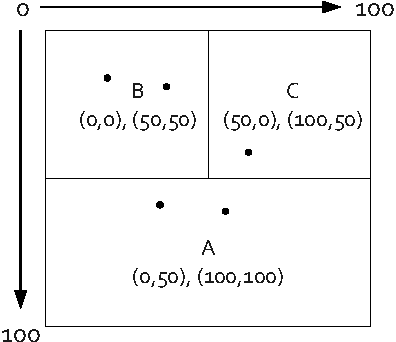
\includegraphics{grafics/can_key_space.pdf}
\caption{Zweidimensionaler Schlüsselraum für CAN}
\label{fig:can_key_space}
\end{figure}

\subsubsection{Routing} 
Die gespeicherte Routinginformation ist bei CAN am geringsten: Jeder Knoten speichert lediglich seine Nachbarn, das sind Knoten deren Zonen angrenzend sind, ab. Über die Zoneninformation jedes Nachbarn wird nun das Routing bestimmt. Eine Nachricht wird über den Knoten geschickt, der aufgrund seiner Zoneninformation näher am Ziel ist.

In \Fref{fig:can_routing} hat Knoten N1 die vier Knoten N2, N3, N4 und N5 als Nachbarn. Knoten N4 hingegen ist nur mit N1 und N5 benachbart. Eine Nachricht von $N1$ zu $K$ wird beispielsweise via Knoten $N5$ geroutet. Eine alternative Route via $N2$ ist gestrichelt dargestellt.

\begin{figure}[htbp]
\centering
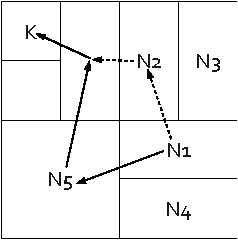
\includegraphics{grafics/can_routing.pdf}
\caption{Routing und Nachbarschaft bei CAN}
\label{fig:can_routing}
\end{figure}

Die durchschnittliche Länge eines Pfades bei $d$ Dimensionen und $n$ Knoten ist $O(d\cdot n^\frac{1}{d})$. Sind die Zonen gleich aufgeteilt, so besitzt jeder Knoten max. $2d$ Nachbarn und die Anzahl an Hops verringert sich auf $O(\frac{4}{d}\cdot n^\frac{1}{d})$.

\subsubsection{Nachbarschaft}
Die Nachbarschaft von CAN wurde bereits im vorigen Abschnitt behandelt. Dank deren Einfachheit ist der Ein- und Austritt von Knoten zwar besonders einfach und tangiert nur wenige Knoten im Netz, jedoch kann auf die Nähe aus Netzwerksicht nur beim Eintritt eines Knotens bei der Wahl seiner Koordinaten Rücksicht genommen werden.

Die Erhöhung der Dimension bedingt eine größere Nachbarschaft und damit, neben einem kürzeren Routing, auch die Möglichkeit mehr Knoten in der Nachbarschaft anzusiedeln. Zusätzlich können in CAN sogenannte \emph{Realitäten} genutzt werden. Dies sind verschiedene CAN-Netzwerke mit unterschiedlichen Hashfunktionen zur Berechnung der Schlüssel. Jeder Knoten und jeder Datensatz ist in jedem dieser Netzwerke vertreten und besitzt einen unterschiedlichen Schlüssel pro Netzwerk. In einem System mit $r$ Realitäten muss ein Knoten demnach $r$ verschiedene Zonen und Nachbarschaften verwalten. Eine Nachricht wird bei jedem Routinghop über die Realität verschickt, welche die kürzeste Route verspricht. Die Nachrichten können durch die verschiedenen Dimensionen \enquote{tunneln}.

\subsubsection{Eintritt und Austritt (Fehlerfall) von Knoten}
Für den Eintritt eines neuen Knotens $n$ muss wieder ein Knoten $b$ aus dem Netz bekannt sein. Eine Koordinate im Schlüsselraum wird n zugewiesen und eine spezielle \texttt{JOIN}-Nachricht via $d$ an die gewählte Koordinate gesendet. Ist diese Nachricht über das normale Routing bei dem für diese Koordinate zuständigen Knoten $d$ angekommen, halbiert dieser seine Zone und weist eine Hälfte dem neuen Knoten $n$ zu. Die Aufteilung der Zonen erfolgt dabei anhand einer Reihenfolge der Dimensionen. Dies vereinfacht die Aufteilungs- sowie die Zusammenführungsprozedur. Letztlich kopiert $d$ alle Daten aus dieser neuen Zone zu $n$. Knoten $d$ schickt $n$ seine Nachbarschaftsinformationen und trägt diesen selbst als neuen Nachbarn ein. Knoten n teilt seine Anwesenheit sofort seinen neuen Nachbarn mit. Der Neueintritt eines Knotens ist damit auf wenige Nachrichten zwischen den Nachbarn begrenzt und beeinträchtigt das übrige Netzwerk nicht. Über periodische \texttt{UPDATE}-Nachrichten halten sich Nachbarn stets aktuell und senden ihre eigenen Nachbarschaftsinformationen an die benachbarten Knoten.

\begin{figure}[htbp]
\centering
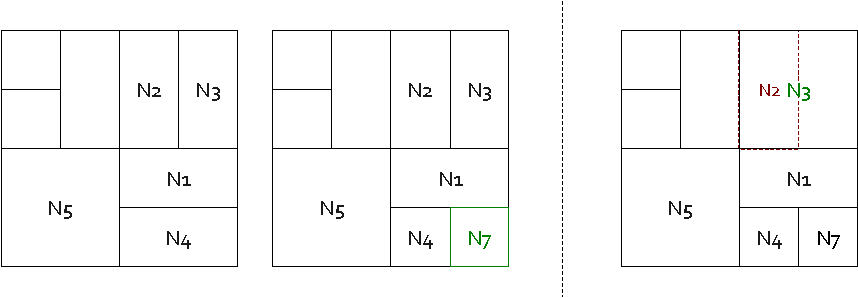
\includegraphics{grafics/can_new_node.pdf}
\caption{Eintritt und Fehlerfall bei CAN}
\label{fig:can_new_node}
\end{figure}

\Fref{fig:can_new_node} zeigt den Eintritt für Knoten N7. Nach Teilung der Zone von N4 verändert sich die Nachbarschaft von N1: Knoten N7 kommt neu hinzu. Die Nachbarschaft von $N1$ ist dann $\{N2, N3, N4, N5, N7\}$. Auf der rechten Seite ist der Ausfall des Knotens $N2$ (rot) dargestellt. Knoten $N3$ ist nun für die vereinigte Zone zuständig.

Ausstehende \texttt{UPDATE}-Nachrichten oder Timeouts weisen auf ausgefallene Knoten hin. Werden diese zum Routen einer Nachricht benutzt, stellt dies keine direkte Beeinträchtigung des Netzes dar, da die Nachricht über einen anderen Nachbarn verschickt werden kann. So könnte N1 auch N2 zum Nachrichtenversand nutzen, wenn N5 ausgefallen wäre (vergleiche \Fref[plain]{fig:can_routing}).

Ein Knoten, der einen ausfallenden Peer entdeckt hat, startet einen Timer, dessen Dauer proportional zur Zonengröße ist. Nach Ablauf sendet der Knoten eine spezielle \texttt{TAKEOVER}-Nachricht an alle Nachbarn des ausgefallenen Knotens\footnote{Dieses Wissen ist durch vorherige \texttt{UPDATE}-Nachrichten bekannt.}. Erreicht eine \texttt{TAKEOVER}-Nachricht einen Knoten, der den Ausfall ebenfalls bemerkt hat, stoppt dieser seinen eigenen Timer, falls seine Zone größer als die des Senders ist. Andernfalls antwortet er selbst mit seiner \texttt{TAKEOVER}-Nachricht. Auf diese Weise wird der Nachbar mit der kleinsten Zone gefunden. Dieser ist nun der neue Besitzer der Zone und fügt seine beiden Zonen zusammen, wie es in \Fref{fig:can_new_node} am Beispiel von N2 und N3 ersichtlich ist. N2 (rot dargestellt) ist ausgefallen und N3 vergrößert seine Zone. N2 ist nun nicht mehr in der Nachbarschaft von N1 enthalten. Es ist möglich, dass ein Knoten Besitzer zweier Zonen wird, welche sich nicht als eine Zone darstellen lassen. Ein Beispiel hierfür ist Knoten N4, der beim Ausfall von N5 dessen Zone übernimmt. Ein Hintergrundprozess defragmentiert solche Zonen und weist Knoten gegebenenfalls neue Koordinaten zu.\\
Eine periodische Auffrischung der Datensätze soll auch hier einen Verlust im Fehlerfall schnell kompensieren.

Möchte ein Knoten l das System verlassen, so sucht er einen Nachbarn mit der kleinsten Zone und sendet diesem seine Daten. Dieser Nachbar informiert nun die alten Nachbarn von l über die geänderte Nachbarschaft.
